\section{Implementation and Evaluation}\label{sec:evaluation}
  
\subsection{Implementation and Methodology}

Its interface is compatible with any model implemented as an {\tt torch.nn.module}. Users can simply wrap their models using this interface and leverage \name-powered DP as they use classic DP. Users do not need to modify their model.  \name-powered DP can be combined with any form of MP including Megatron-LM~\footnote{\url{https://github.com/nvidia/Megatron-LM}}.

\subsection{Speed and Model Size}
Figure~\ref{fig:billion_parameter_speedup} shows throughput per GPU for varying model sizes using \name-100B with MP versus using Megatron MP alone.

\begin{figure}[t!]
   \begin{center}
   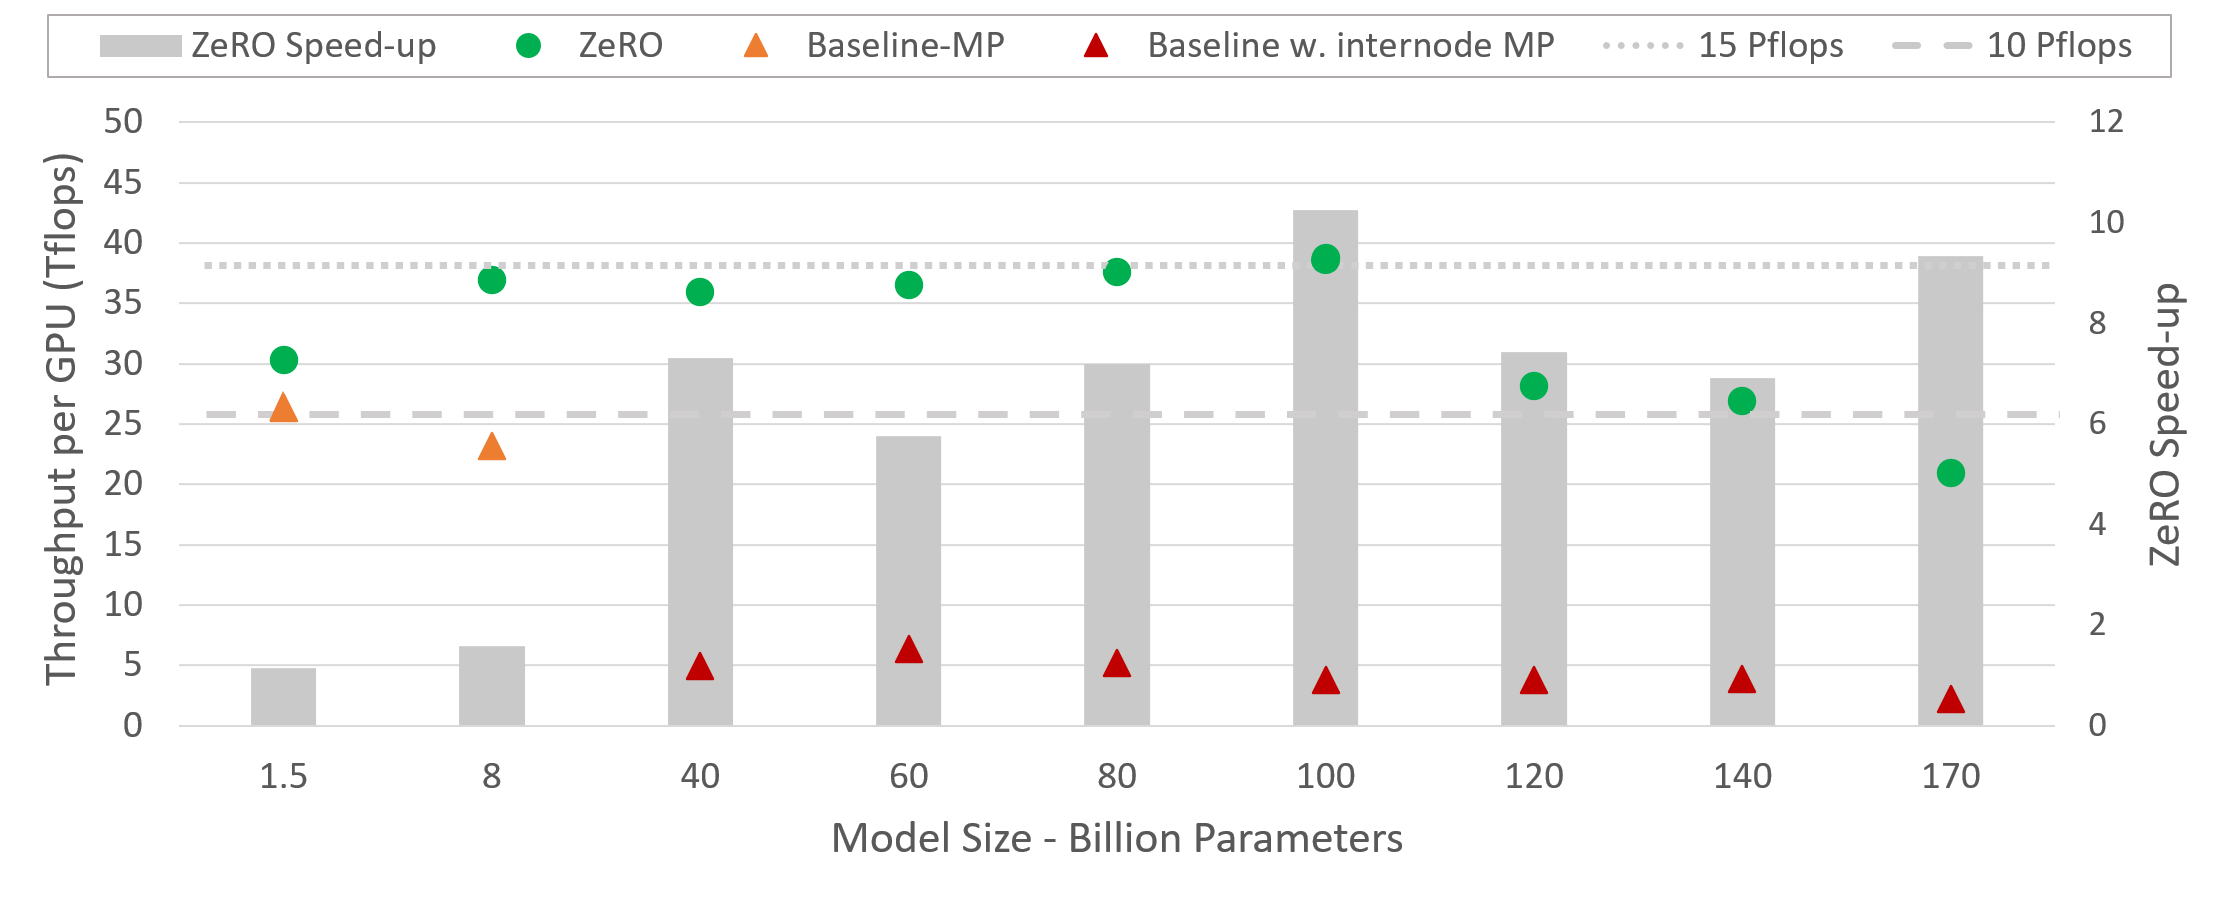
\includegraphics[width=1.0\columnwidth]{model_size_and_speedup.PNG}
   \caption{\name training throughput and speedup w.r.t SOTA baseline for varying model sizes.  For \name, the MP always fit in a node, while for baseline, models larger than 40B require MP across nodes.} 
   \label{fig:billion_parameter_speedup}
   \end{center}
\end{figure}

For \name-100B, the slight reduction in performance beyond 100B is due to lack of enough memory to run larger batch sizes.

\subsection{Super-Linear Scalability}
\name-100B demonstrates super-linear scalability for very large model sizes. Figure~\ref{fig:hyperscale_60B} shows scalability results for a 60B parameter model going from 64 to 400 GPUs and we expect this trend to continue further for more GPUs.

\begin{figure}[t!]
   \begin{center}
   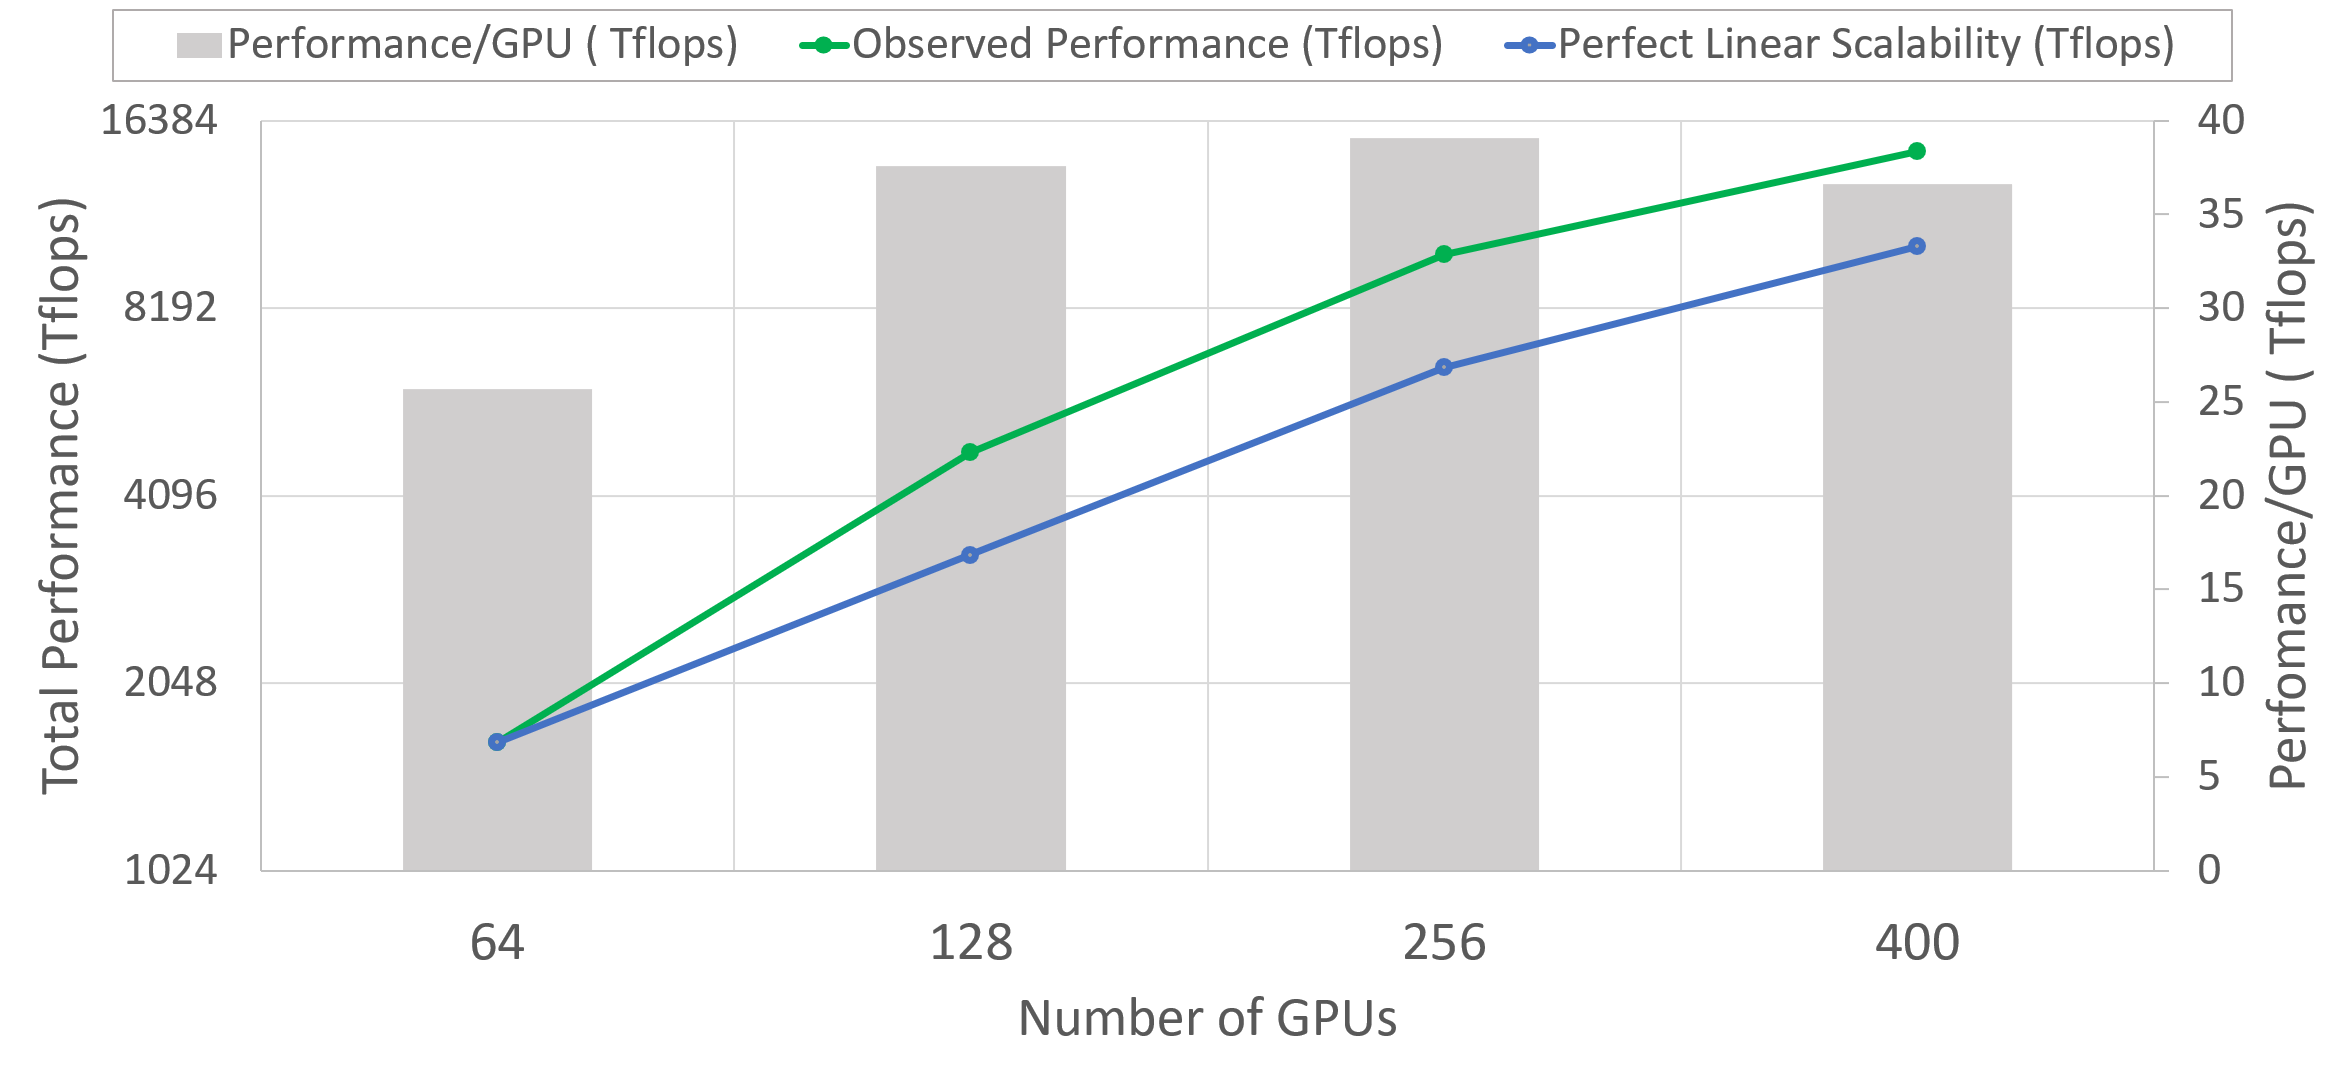
\includegraphics[width=1.0\columnwidth]{hyperscale_60B_model_v2.PNG}
   \caption{Superlinear scalability and per GPU training throughput of a 60B parameter model using \name-100B.} 
   \label{fig:hyperscale_60B}
   \end{center}
\end{figure}

\subsection{Democratizing Large Model Training}
Figure~\ref{fig:dp_tput} shows that \name-100B can train models with up to 13B parameters without MP on 128 GPUs, achieving throughput over 40\,TFlops per GPU on average.

\begin{figure}
   \begin{minipage}[b]{0.55\columnwidth}
    \centering
       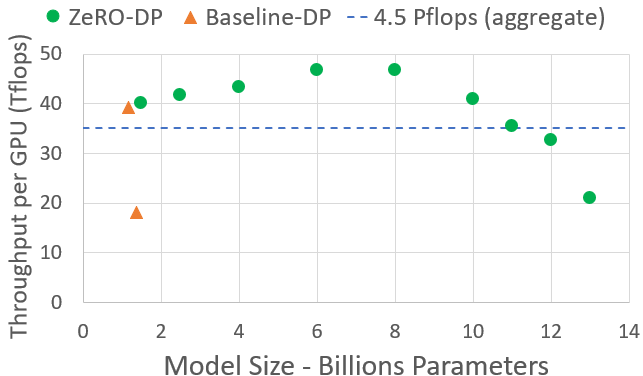
\includegraphics[width=\textwidth]{max_data_parallel_throughput.PNG}
        \caption{Max model throughput with \name-DP.} \label{fig:dp_tput}
   \vspace{0.04in}
   \end{minipage}
   \quad
   \begin{minipage}[b]{0.4\columnwidth}
    \centering
       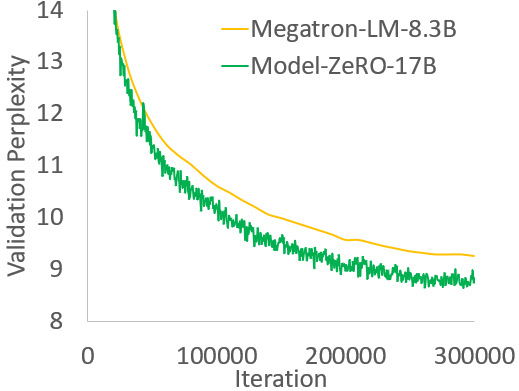
\includegraphics[width=\textwidth]{turing_nlg_17B.PNG}
        \caption{SOTA Turing-NLG enabled by \name.} \label{fig:turing_nlg_17B}
      \vspace{0.08in}
   \end{minipage}
\end{figure}

\subsection{Turing-NLG, the SOTA language model with 17B parameters}
Turing-NLG was trained end-to-end using \name-100B and Figure~\ref{fig:turing_nlg_17B} shows the validation perplexity over 300K iterations compared to previous SOTA, Megatron-LM 8.3B parameter model.